\chapter{Background}
\label{chap3}

This chapter describes what glitch attacks are, why developers need to protect their devices from them and their current limitations. The \textit{CV32E40S} RISC-V core by the OpenHW group is also introduced, and the potential benefits of removing some of its security features are investigated. 

\section{What are glitch attacks?}
\label{sec:glitch_attacks}

Glitch attacks, also known as hardware fault injection, are a sophisticated form of hacking aimed at exploiting vulnerabilities in hardware systems. The primary objective is to disrupt normal execution to bypass security features in order to gain access to sensitive data, bypass authentication protocols or undermine cryptographic operations. 

Glitch attacks can be divided into two main categories: invasive (e.g., decapsulating the chip\cite{intro_to_hw_hacking}) and non-invasive attacks (e.g., electromagnetic fault injection (EMFI), voltage- and clock-glitching). Often times software and firmware security measures can only protect against non-invasive glitches, as protecting from invasive glitches often require hardware modifications\cite{glitchresistor}. Due to the nature of invasive attacks, it is beyond the scope of this project to defend against them. This is because these often aim at tampering with Read-Only Memory (ROM) or Boot-loaders on Printed Circuit Boards (PCBs), and are not effective against more complex systems like a Central Processing Unit (CPU) or a System on Chip (SoC). Therefore, protecting against these attacks is the responsibility of other components than the one discussed in this project. 

\subsection{Non-invasine glitch attacks}
\label{sec:non_invasive}

Non-invasive glitches can be performed as long as an attacker has access to a device. However, there is quite a lot of procedural vulnerability discovery that has to be done before an attack can be performed. In the case of Electromagnetic Fault Injection (EMFI) the chip has to be repeatedly exposed to electromagnetic interference during execution, to then determine which areas are most vulnerable to attacks\cite{emfi_injection}. An example of such probing being performed on the BCM2837 SoC can be seen in \autoref{fig:emfi_map}\cite{emfi_injection}. 

Voltage- or clock-glitching can be performed as long as there is some way to access these signals externally. Voltage-glitching often requires the removal of power filtering capacitors to gain more fine-grained control over a processor's voltage input. However, both of these methods require very precise timing by an attacker. This is why specialized tools such as the \textit{ChipWhisperer}\cite{chipWhisperer} were made, as they allow for extremely accurate fault-injection. These days it is also possible to perform effective glitch attacks with simple components in conjunction with a cheap Field Programmable Gate Array (FPGA) which outputs precise triggers as shown in\cite{hole_in_soc}. 

\begin{figure}[h!]
    \centering
    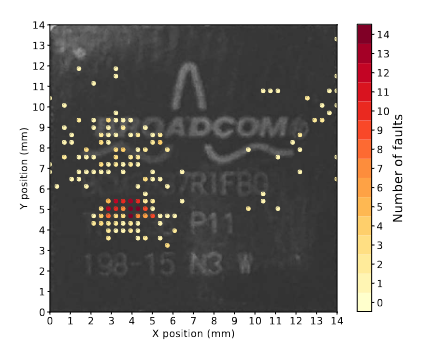
\includegraphics[scale=0.5]{docs/images/emfi_error_map.png}
    \caption{EMFI BCM2837 sensitivity map (dot size is not corralated with probe size.)\cite{emfi_injection}.}
    \label{fig:emfi_map}
\end{figure}

Voltage-glitching is performed by momentarily dropping the supply voltage during execution of critical operations. Clock-glitching is performed by altering clock timing to violate setup and hold time requirements of the hardware\cite{intro_to_FI}. The results of glitching cannot always be predicted, however they mainly result in skipped or repeated CPU instructions, incorrect evaluation of CPU instructions or corrupt reads from memory devices\cite{intro_to_FI}. In general these faults can occur at any stage in the execution pipeline. A typical application for these types of glitches is to skip some sort of signature verification in a bootloader or other security module. Take for instance the example code shown in \autoref{fig:glitchable_code}. In this code a boot image is fetched. The result code of this operation is then checked to see whether the correct image was fetched, or if an error occurred. In the case of an error, the program is stuck in in an infinite loop and if not the boot process can continue. From the figure one can observe that there exists a number of weak points that can be exploited. Because of this hardware designers implement things like \textit{Program Counter Hardening} (PCH) to check for instruction skips by comparing current and expected PC values, and \textit{Error Correcting Code} (ECC) to validate data integrity in registers. However, while these features would stop an attacker in this example, what if the attacker finds a way to boot with the wrong PC and start at the 'do\_boot' instruction? In this case we would need to develop a new form of protection with a greater fault detection coverage. Such a solution is discussed in this project in the form of a dual-core lockstep mechanism. 

\begin{figure}[h!]
    \centering
    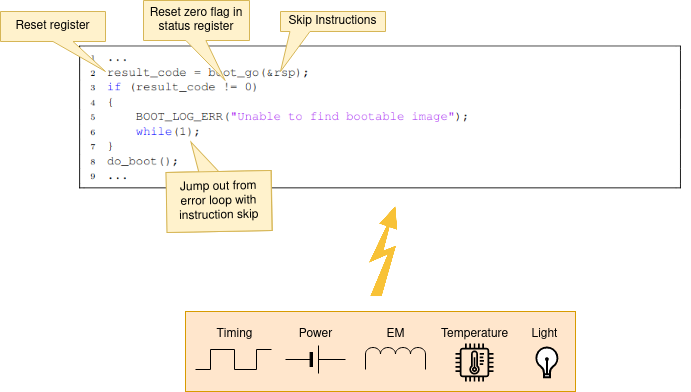
\includegraphics[width=0.75\textwidth]{docs/images/glitch_attack_whole_system.png}
    \caption{Example of code that can be glitched with common attacks. \footnote{Figure inspired by one found in “Fault Attacks on Secure Embedded Software:
Threats, Design and Evaluation”, Bilgiday Yuce, Patrick Schaumont,
Marc Witteman}}
    \label{fig:glitchable_code}
\end{figure}

% Glitch attacks have over recent years become a more common and greater threat. Due to the nature of how these attacks are carried out, they are often a very affordable way to exploit hardware. Attackers have easy access to open source resources like the the 'ChipWhisperer Lite' which allows for easy access to hardware glitching tools as well as side channel analysis\cite{chipWhisperer}. In addition to this, FPGAs can be used to inject precisely timed faults as long as an attacker has access to the supply voltage or clock on a chip\cite{hole_in_soc}. 

\section{The need for glitch protection}

Within the world of CPU design the two biggest architectures are ARM and x86 (produced by Intel and AMD). Most of the devices we us every day has one of these types of chips inside them, and because of this they also implement several security features to prevent glitch attacks. For ARM processors this includes among other things the \textit{TrustZone} which provides hardware-enforced isolateion between trusted and non-trusted software, as well as built in physical attack protection\cite{arm}. The 12th gen x86 processors produced by Intel have a Tunable Replica Circuit (TRC), which uses hardware-based sensors to explicitly detect circuit-based timing failures that occur as the result of an attack\cite{intel}.  

Unfortunately, for many years the world of CPU design has been hidden from the public due to the strict secrecy producers have around their products. While this limits what the public can know, it also means that a potential hacker would have a much harder time if they wished to exploit how the ISA of a chip is designed. Due to the nature of open source projects, this is a larger vulnerability for products based on a RISC-V architecture. An example of direct exploitation of the architecture was shown during the 'DEFCON' conference in 2019\cite{isa_exploit}. Here it was demonstrated that triggering an exception during boot of a RISC-V chip would lead to an 'exception loop'. This was because the Machine Trap Vector (MTVEC) had no base address before boot (e.g., it was set to 0x0). Pointing to this address is permitted in the ISA, and doing so will trigger an exception. This means that triggering an exception before boot leads to the exception handler pointing to an illegal address, which again triggers an exception and this continues forever. Handling of exceptions happens first at the highest privilege mode (Machine mode), which means that the chip is also stuck in this mode. 

The RISC-V architecture is designed with some key security features in mind. One of these are the previously mentioned privilege levels. These are in descending order: machine (M-mode), hypervisor (H-mode), supervisor (S-mode) and user mode (U-mode). A higher privilege mode can access all the functions used in a lower privilege mode\cite{source2}. Other key security features in the RISC-V architecture are the physical memory protection (PMP), which controls memory accesses, and the use of a trusted execution environment (TEE). The TEE is meant to ensure that code and data loaded into this environment are protected with respect to confidentiality and integrity. However, as shown in (Nashimoto et al. 2020) the integrity of TEEs can also be bypassed using clock-glitching\cite{source2}.

%\section{Previous Approaches to glitch protection}
\section{CV32E40S by the OpenHW group}
\label{sec:cv32}

The previously mentioned security measures do a decent job at protecting hardware against malicious attacks. However, the need for more security features has been required and therefore the \textit{OpenHW} group developed the \textit{CV32E40S}. This is a 4-stage in-order 32-bit RISC-V processor core with the main intention of ensuring secure operation\cite{cv32e40s_manual}. This core has the same privilege modes and PMP as described to ensure a TEE. There are however implemented extra security features and an Instruction Set Extension (ISE), \textit{Xsecure}. The CV32E40S started out as a fork of the CV32E40P which is another RISC-V processor made by the OpenHW group. The top-level block diagram of the CV32E40S core is shown in \autoref{fig:cv32e40s_block}. From the figure one can see that the architecture of this core is much like any other RISC-V core, with a clear Instruction Decode, Instruction Fetch, Execute and Write Back stages. The extra security features of this core are a PCH module in the IF stage (not shown in figure), ECC in the register file in the ID and CSR Hardening in the EX stage. 

%The top-level block diagram of the cores is shown in \autoref{fig:core_comparison_block}. From the figure we can see that the main difference on the top level is the PMP and the Physical Memory Attribution (PMA), which allows for compile time attribution of the physical memory map.

% \begin{figure}[h!]
% \centering
%     \subfigure[CV32E40P\cite{cv32e40p_manual}.]{%
%     \label{fig:cv32e40p_block}%
%     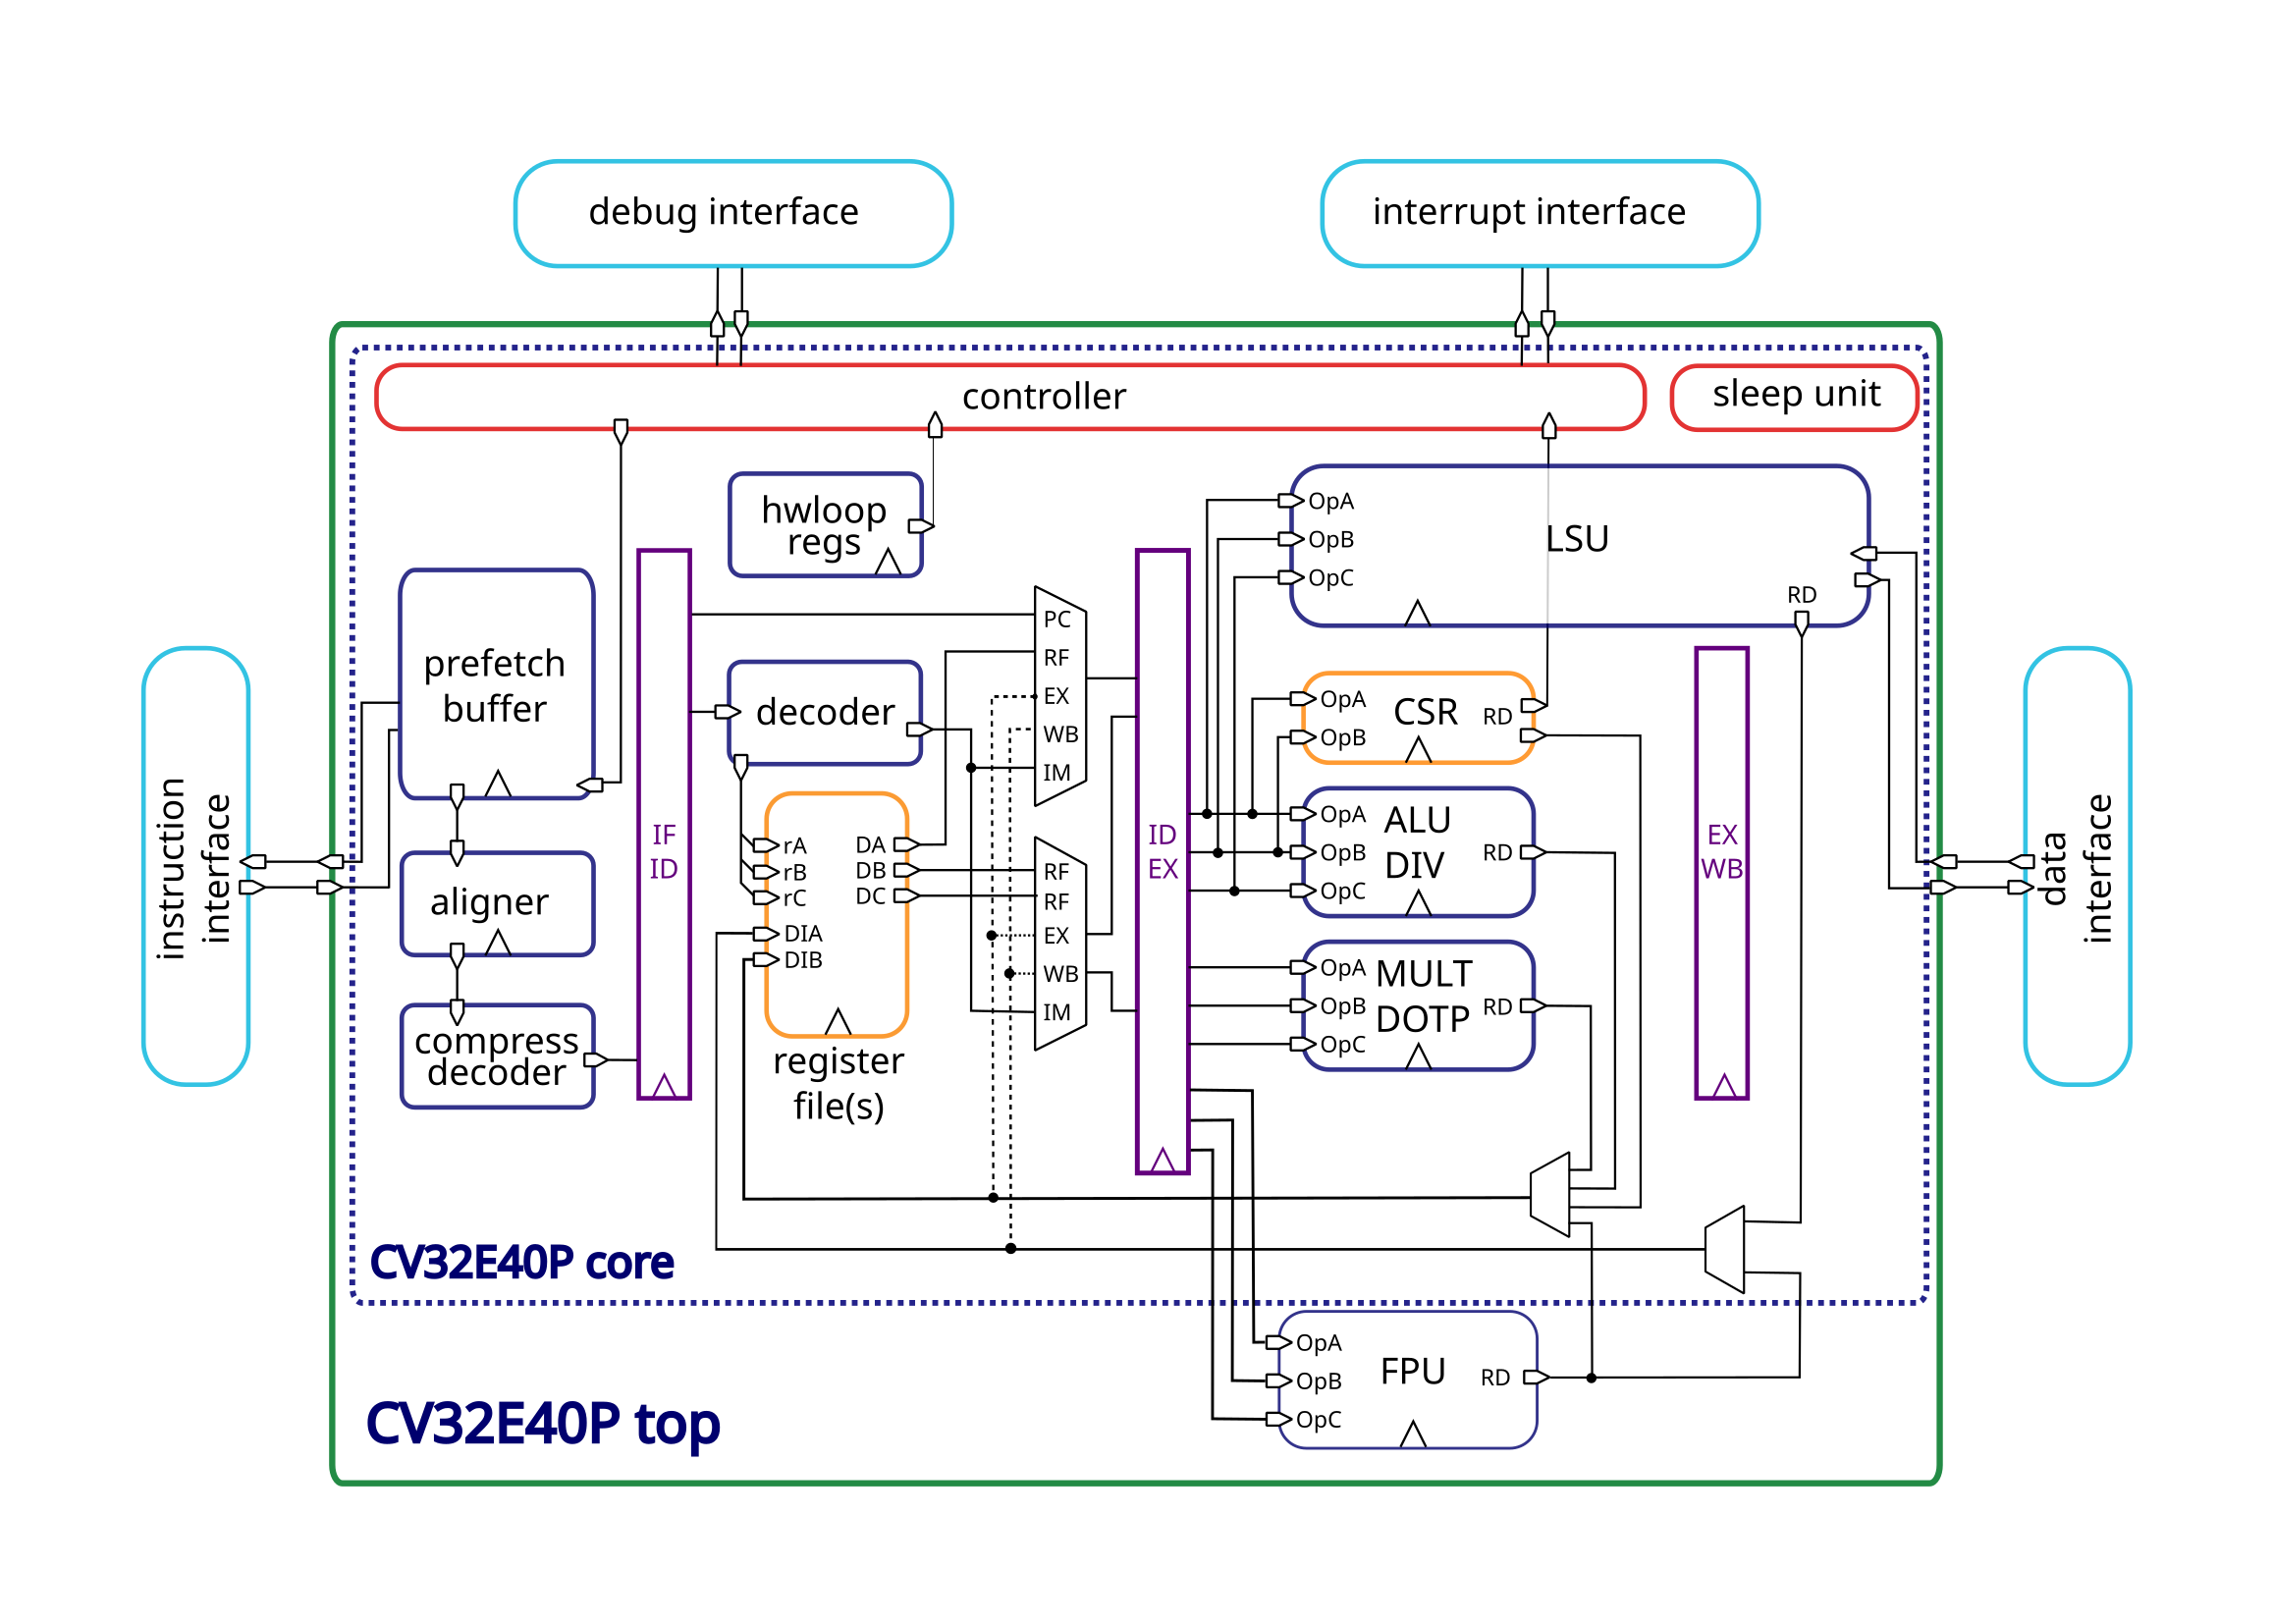
\includegraphics[width=0.47\textwidth]{docs/images/CV32E40P_Block_Diagram.png}}%
%     \qquad
%     \subfigure[CV32E40S\cite{cv32e40s_manual}.]{%
%     \label{fig:cv32e40s_block}%
%     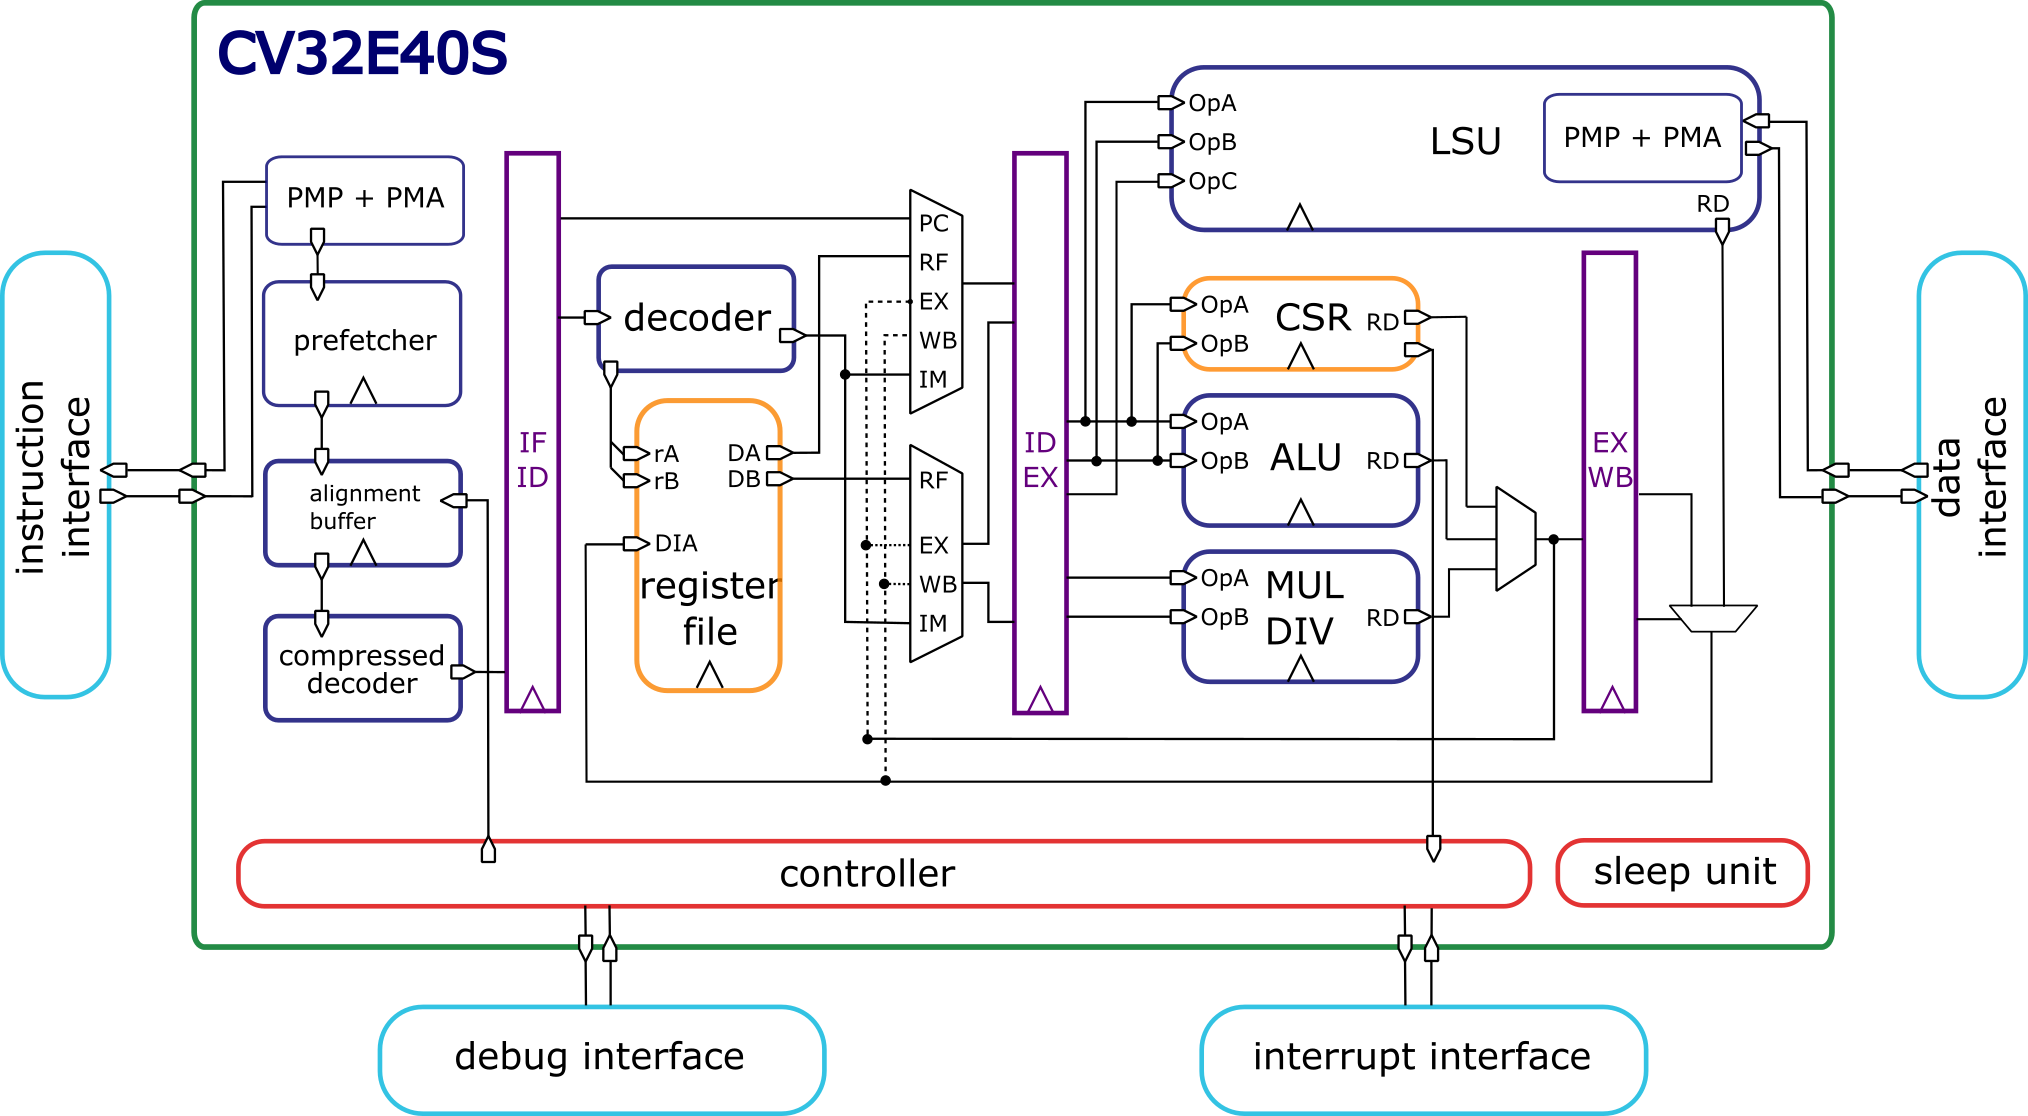
\includegraphics[width=0.47\textwidth]{docs/images/CV32E40S_Block_Diagram.png}}%
%     \caption{Comparison of Top-Level Block Diagram for CV32E40S and CV32E40P.}
%     \label{fig:core_comparison_block}
% \end{figure}

\begin{figure}[h!]
    \centering
    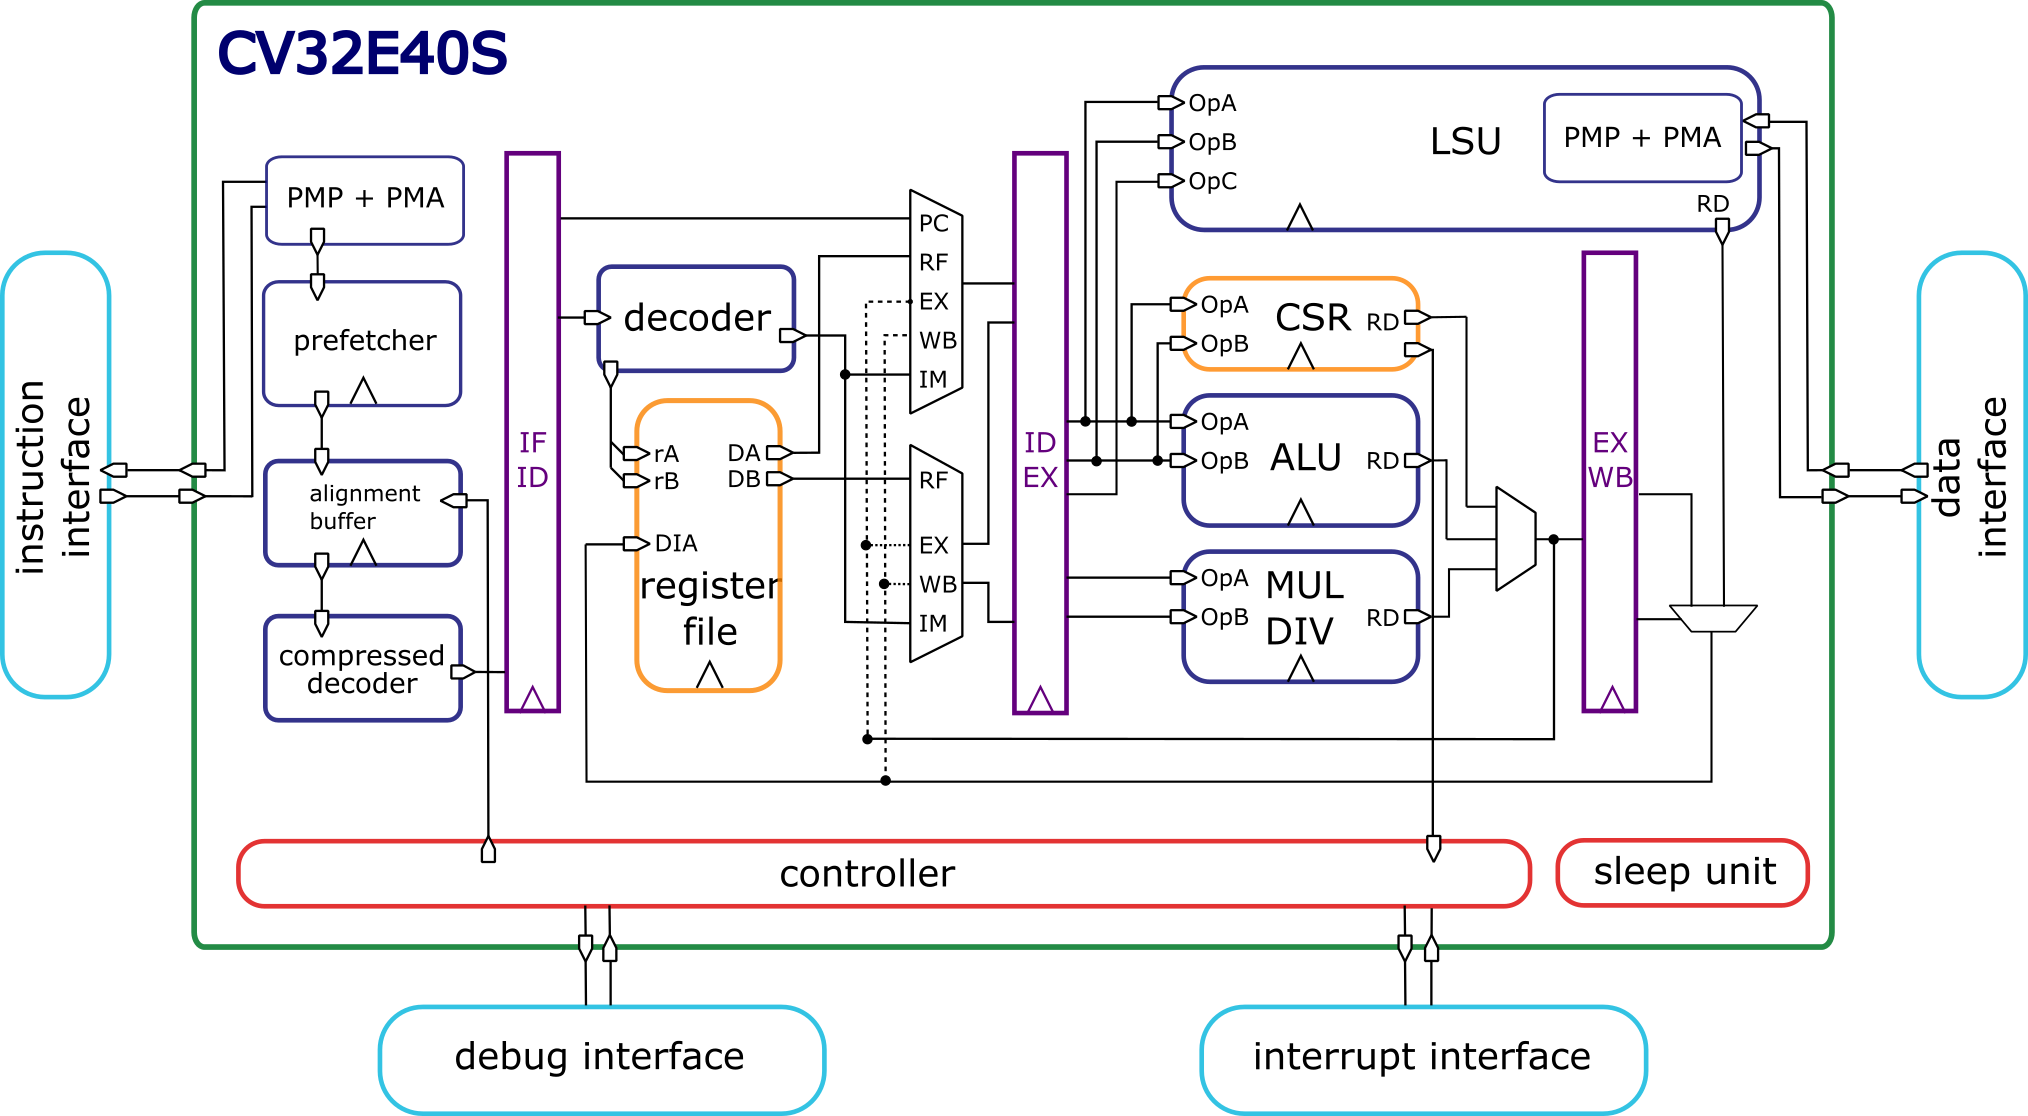
\includegraphics[width=0.6\textwidth]{docs/images/CV32E40S_Block_Diagram.png}
    \caption{CV32E40S top-level block diagram\cite{cv32e40s_manual}.}
    \label{fig:cv32e40s_block}
\end{figure}

\subsection{Xsecure Extension}
\label{sec:xsecure}

\textit{Xsecure} is an ISE that adds extra security functionality within many of the different sub modules of the core. These security features are meant to deter side-channel attacks through the use of \textit{data independent timing}, \textit{dummy instruction insertion} and \textit{random instructions}\cite{cv32e40s_manual}. While these features will increase execution time, they cannot easily be removed with the use of a dual core setup. This is because preventing side-channel attacks is less about redundancy and more about making the power usage or execution time of a processor unpredictable. 

The extension also adds specific security features to prevent glitch attacks. These include: \textit{Register file ECC}, \textit{Hardened PC} and \textit{Hardened CSRs} among other things. These features can potentially be removed in favour of a dual core lock-step mechanism. Removing only these features without also affecting the core as a whole is quite complicated. However, to give some insight into the resource usage and added execution time for these sub-modules, the core has been simulated and synthesized both with and without \textit{PC Hardening}. When simulation of the core is done, a simple \textit{hello-world} example is run, shown in \autoref{app:helloworldC}. From simulation of both cores it is shown that the core requires \textbf{9} extra clock cycles when using \textit{PC-hardening} as can be seen in \autoref{tab:simulation_cc}. The instruction trace file for this test shows that there are \textit{11875} instructions executed. From the documentation about the core, it is explained that \textit{jumps} as well as \textit{branches} that are not taken will require one extra clock cycle due to \textit{PC-hardening}. From \autoref{fig:instr_occ} it can be observed that the program contains approximately $\approx$ 3000 branch and jump instructions combined. This means removing the \textit{PC-hardening} should reduce the total amount of clock cycles by minimum 1.6\% (if all jumps and branches are taken) and a maximum of 16\% (if all jumps are taken but no branches). 
The reason for this discrepancy between the documentation and simulation results is that the core contains features to prevent side-channel attacks as well as glitch attacks. One of these features is \textit{Data Independent Timing} (DIT) which leads to all branches in a program being taken (branches that would not normally be taken are immediately followed up by killing of the fetch and decode stages). \autoref{tab:simulation_cc} shows the clock cycles needed with DIT enabled and disabled. From this it is possible to see that \textit{PC-Hardening} actually adds \textit{843} clock cycles which represents an increase of approximately 5\%. 

\begin{table}[h]
\centering
\caption{Number of clock cycles needed to simulate the program in \autoref{app:helloworldC} with and without \textit{PC-Hardening}.}
\label{tab:simulation_cc}
\begin{tabular}{c|cc}
\toprule 
Data Independent Timing & With PC-Hardening & Without PC-Hardening \\
\midrule
\rowcolor{black!20} enabled & 18289 & 18280 \\
disabled & 17313 & 16470 \\
\bottomrule
\end{tabular}
\end{table}

\begin{figure}[h!]
    \centering
    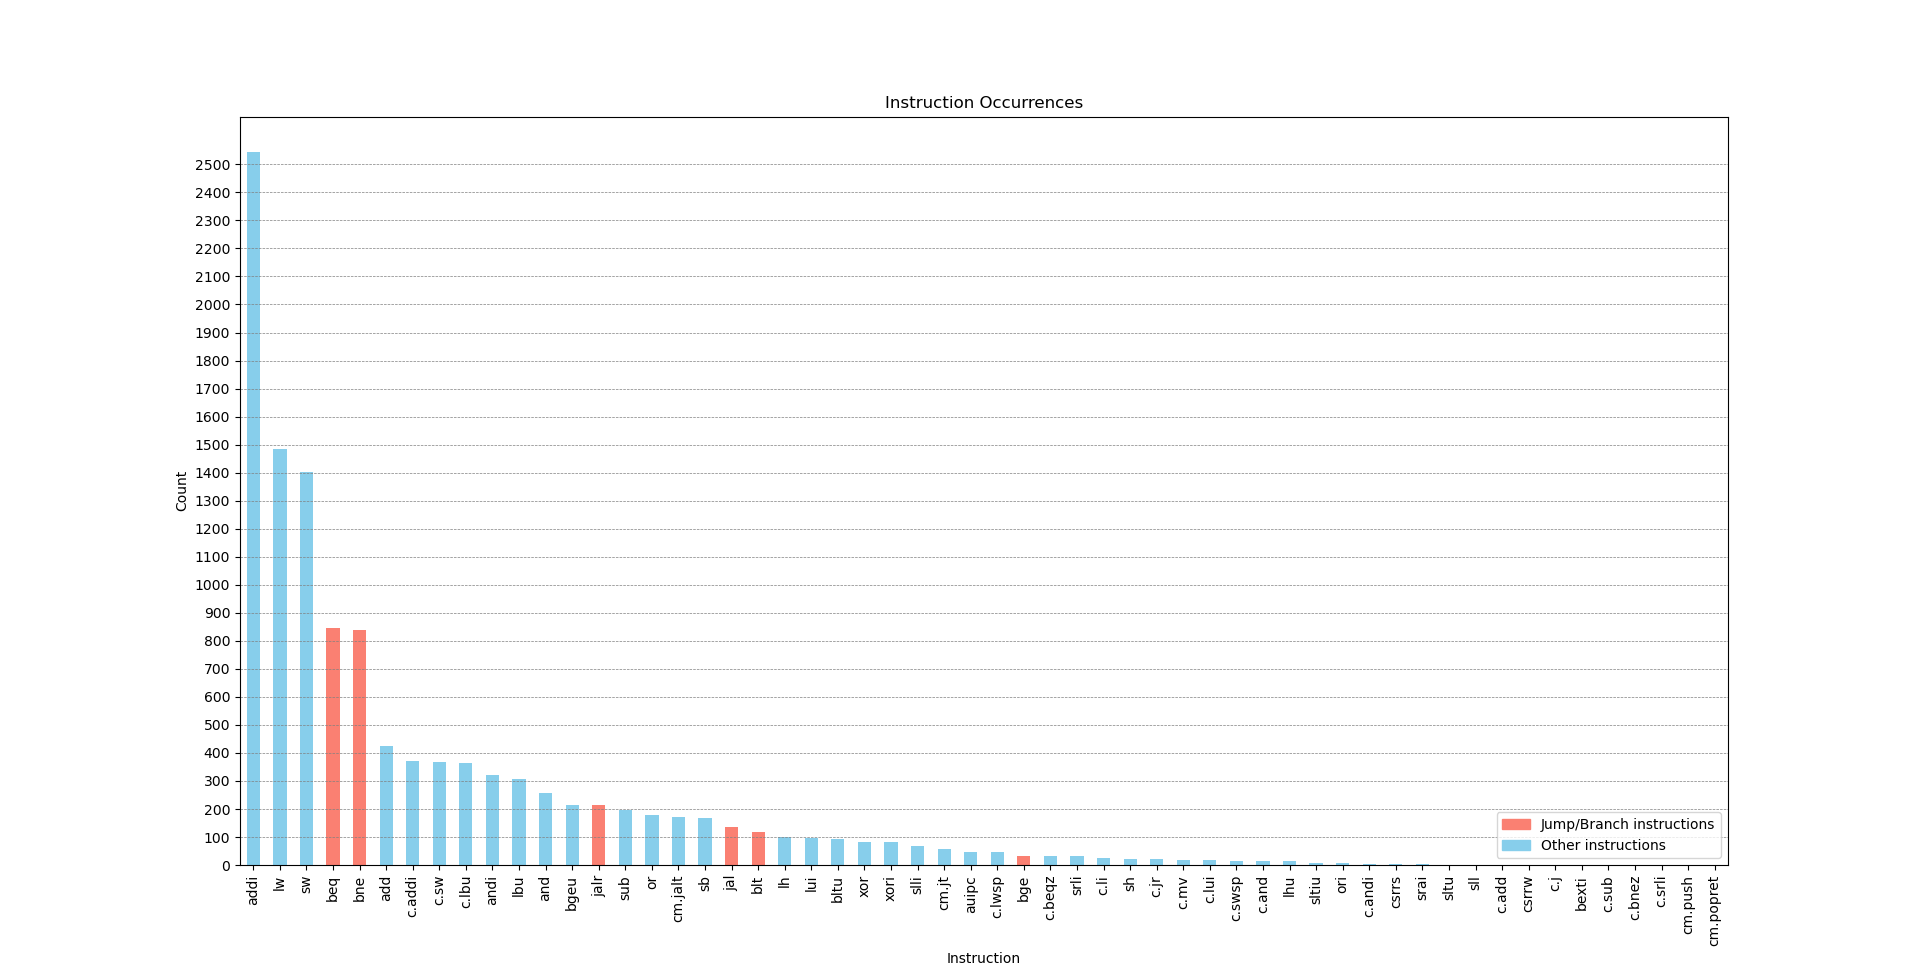
\includegraphics[width=\textwidth]{docs/images/instruction_occurances_all_legend.png}
    \caption{All instructions in the generated assembly for the \textit{hello-world}\autoref{app:helloworldC} example, and the amount of calls for each instruction.}
    \label{fig:instr_occ}
\end{figure}

\autoref{tab:synth_ppa} shows synthesis results of both cores. The \textit{PC-Hardening} will add a bit to the total area and power usage. However, the module is quite small and the increase in resource usage is not very significant. 

\begin{table}[h]
\centering
\caption{Synthesized resource usage with and without \textit{PC-Hardening}.}
\label{tab:synth_ppa}
\begin{tabular}{ccc}
\toprule 
& With PC-Hardening & Without PC-Hardening \\
\midrule
\rowcolor{black!20} \textbf{area[$pm^2$]} & 63164.38 & 61757.916 \\
\textbf{power[$W$]} & 1.12163mW & 1.10450mW \\
\bottomrule
\end{tabular}
\end{table}

\section{Limitations of glitch protection}
\label{sec:limits}

Despite greatly increasing the hardware security of devices, many glitch protection methods can have some common limitations. For instance the coverage of protection can often be incomplete. This means that designers often only focus on the most critical glitches, and can therefore sometimes overlook seemingly insignificant glitches that might break the system. For instance, a designer could implement a robust check to see whether the program counter has been modified during execution. However if an attacker glitches the program counter on boot, it could go undetected by the checker mechanism. 

In general, glitch protection mechanisms will add to both the area and power consumption of a chip. Often the added area also comes from components that are logically redundant. In addition there will potentially be quite a lot of latency added. As previously described in \autoref{sec:xsecure}, the \textit{PC-hardening} module will add one extra cycle per jump or branch that is not taken. From \autoref{fig:instr_occ} it can be seen that even in a very simple program the potential for added latency is big. However, most of the potential performance gain that can be achieved from removing the \textit{Xsecure} features is mitigated by the side-channel safety features, which can not be removed. 

From simulation and synthesis of both cores it is obvious that the argument for using a dual-core lockstep mechanism cannot be made solely on resource usage and performance gain alone. However, the main advantage will be the coverage and robustness gained. To test this claim, the regular and dual-core setups will both be subjected to several different glitch attacks that will take place in different parts of the pipeline. The quality of the solution will then be determined by how effective each setup is at responding to the attack. 

\section{Problem Definition}

The openHW group has developed an instruction set extension (ISE) 'Xsecure' which contains several extra features aimed at stopping side-channel attacks as well as glitches. To prevent glitches the extensions introduces ECC for the registers and hardening of both the PC and the CSRs. These additions can slow down the performance of the CPU, increase the power usage and increase the over all complexity of the core. This paper researches the possibility of using dual RISC-V cores and comparing the entire state of both cores to provide redundancy and thereby glitch protection, without significantly impacting the power, performance and area (PPA) in a negative way. 

The current way of doing glitch protection that is used by 'Xsecure' also allows the user to sometimes get a specific error message saying where and what things went wrong. This feature is however not able to do this for all major alerts or errors. The proposed dual core setup might be able to give detailed errors every time as it is possible to know exactly which area of the cores that are not coinciding. 

Introducing a dual-core setup offers potential glitch protection via redundancy. However, the feasibility, overheads, synchronization mechanisms, and actual effectiveness of such a strategy needs thorough examination. In addition, the strategies for detection of a glitch, switch-over mechanisms, and potential recovery strategies need to be explored. An exploration of where and how glitches typically affect RISC-V cores is crucial. From other literature it is apparent that most glitches are induced outside of the CPU pipeline itself, and instead on larger area intensive components like data busses or register files/caches\cite{emfi_injection}. Because it is not feasible to validate the state of caches and register files at all times it is necessary to explore whether a dual core setup will be able to stop or register these types of glitches also. 


% \begin{itemize}
%     \item High logic cost 
%     \item Slower execution of certain pipeline stages
%     \item Lower throughput 
%     \item A typical way of doing fault injection is though EMFI attacks which target larger components like caches or other memory components.
%     How can we prevent these? Comparing the state of the entire chache is not viable, and thus we must allow a fault to persist in 
%     memory untill it is read or used in one of the cores.
% \end{itemize}

%\textbf{I NEED TO SIMULATE THE CORE WITH AND WITHOUT PC-HARDENING AND CSR-HARDENING TO SEE THE DIFFERENCE IN PPA}
%\textbf{I need to create a c program that has some code that is easily glitchable that represents a real world safety feature. This could be an infinite while loop, where the aim is to break out of this loop using a glitch. To achieve this I can either make a module whose sole purpose is to glitch a register and then make this glitchin happen radomly. Or i can induce som form of clock-glitching. This might not be possible in simulation as the setup / hold times will not be realistic. Voltag eglitching is also not possible as I dont havee access to the supply voltage of the system.}

% \textbf{TODO:}
% \begin{itemize}
%     \item Run simulation of core with and without xsecure extension 
%     \begin{itemize}
%         \item Find out where the Xsecure extension is being enabled from. Maybe this is in the documentation. 
%     \end{itemize}
%     \item Run synthesis of core (with and without xsecure extension) 
%     \begin{itemize}
%         \item Power estimation 
%         \item LUTs and Area 
%     \end{itemize}
%     Detail the program that is running when these tests are performed(mostly for simulation)
%     \item Detail how dual cores could work in theory to improve things 
%     \item Describe the tests that will be performed to simulate glitching
%     \item Describe test program that will be running on the core (an infinite while loop to simulate some form of security check)
%     \item Describe the odule that will be implemented to simulate a glitch attack.
% \end{itemize}

% \section{Simulation data}
% \subsection{Clock cycles}
% With PC hardening disabled: 6 cycles

% \subsubsection{Hardened CSR}

% \section{The dual core proposition}
% \section{Rationale for this study}